%%%%%%%%%%%%%%%%%%%%%%%%%%%%%%%%%%%%%%%%%%%%%%%%%%%%%%%%%%%%%%%%%%%%%%%%%%%%%%%%
\chapter{Architecture and Methods}\label{ch:architecture}
%%%%%%%%%%%%%%%%%%%%%%%%%%%%%%%%%%%%%%%%%%%%%%%%%%%%%%%%%%%%%%%%%%%%%%%%%%%%%%%%

In this chapter, we will present our tool which aims to fill the gaps addressed in chapter~\ref{ch:introduction}. \textit{SIMITAR} is an acronym for \textbf{\textit{SnIffing, ModellIng, and TrAffic geneRation}}\footnote{A Scimitar or Scymitar is curved sword, originating in the Middle East\cite{scymitar-sword}.}. This acronym summarizes its operation.
SIMITAR is a traffic generator able to \textbf{\textit{learn}} features of real traffic automatically, and reproduce synthetic traffic similar to the original. It records a model for the traffic in an \acrshort{XML}\footnote{Extensible Markup Language (XML) is a markup language that defines rules for storing and processing hierarchical data\cite{web-xml}.} file we call the \textit{Compact Trace Descriptor}(CTD file) as input-data SIMITAR can use, \textit{pcap} files or real-time captures. 

\begin{figure*}[ht!]
    \centering
    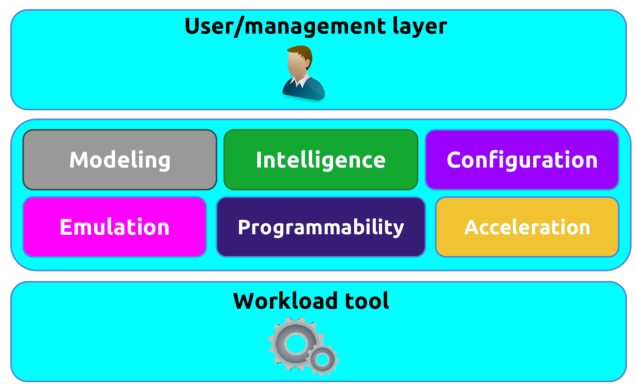
\includegraphics[height=2.4in]{figures/ch1/layer-diagram}
    \caption{ Architecture conceptual idea: a toll to automatize many tasks on traffic modelling and generation.}
    \label{fig:layer-diagram}
\end{figure*}

In figure~\ref{fig:layer-diagram} we abstract our stated concepts in a layer model diagram. Our tool works as an intermediate layer which offers traffic \textbf{\textit{modeling}}, \textbf{\textit{configuration}}, \textbf{\textit{emulation}}, and \textbf{\textit{programmability}}. In the figure, we also include packet acceleration\footnote{Packet acceleration is a concept introduced by DPDK\cite{web-dpdk}, which means kernel by-pass. Packet acceleration optimizes the packet processing, and therefore traffic generation, enabling higher throughput rates.}, which is not implemented yet but discussed as future work, in chapter~\ref{ch:conclusion}.  We are going to refer to the underlying workload tool as the packet generator engine and it is used via API by SIMITAR. 

We are also introducing the concept of \textit{programmability}. The user may create custom traffic, creating the \textit{Compact Trace Descriptor}, following its template. The idea is that he or she can create custom traffic in a platform agnostic way, without having to study any documentation, and implement any script or program.  Using a component methodology, we uncouple the packet generation, from the data collection and parameterization process. We developed it using the factory design pattern\footnote{Design patterns are abstractions that aim to help the implementation and systems structuring\cite{web-design-patterns}.} to make the extension easy for any packet generator engine. 

We abstract its whole operation cycle in figure~\ref{fig:cycle-of-operation}. Our tool collects packet data from live captures or pcap files. It then breaks down the traffic into flows and uses the data to generate parameters for our traffic model. Finally, SIMITAR provides these parameters to a packet generator engine and controls the packet injection.

% cycle of operation
\begin{figure*}[ht!]
        \centering
        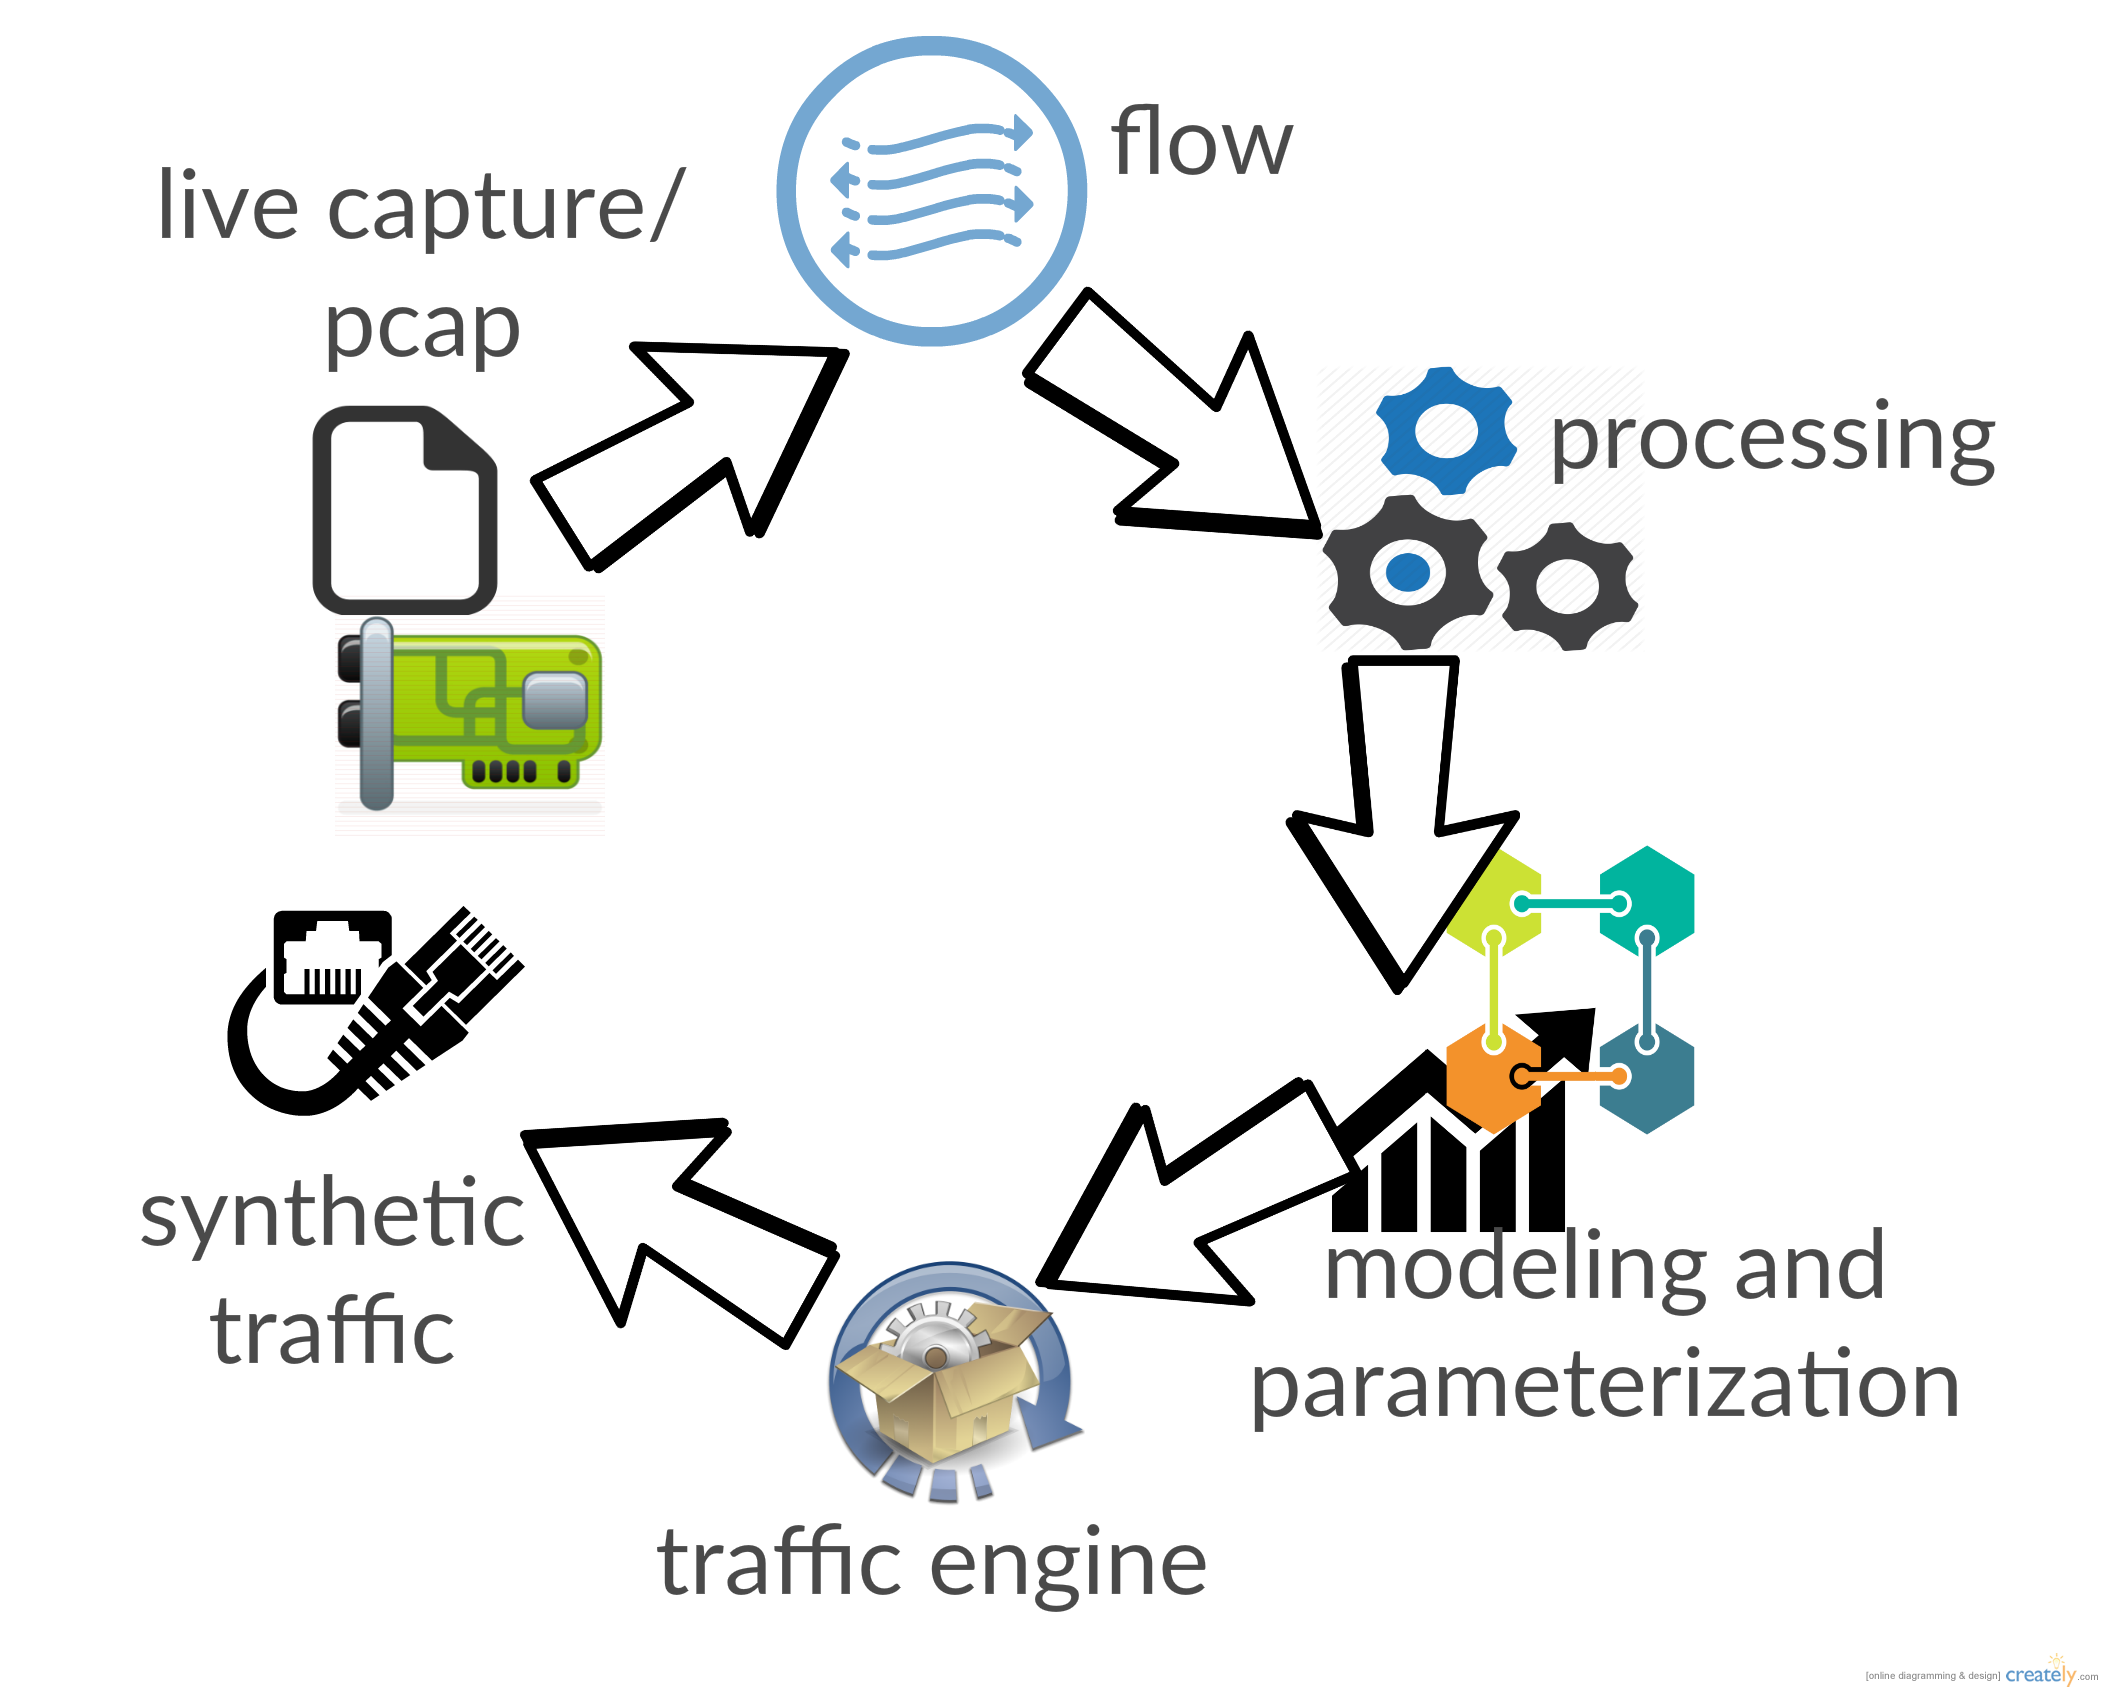
\includegraphics[height=3.0in]{figures/ch3/digram-project-cycle}
        \caption{This figure represents an operation cycle of SIMITAR, emphasizing each main step: sniffing, flow classification, data storing, data processing and fitting, model parameterization,  and synthetic traffic generation.}
    \label{fig:cycle-of-operation}
\end{figure*}

%%%%%%%%%%%%%%%%%%%%%%%%%%%%%%%%%%%%%%%%%%%%%%%%%%%%%%%%%%%%%%%%%%%%%%%%%%%%%%%%
\section{SIMITAR Architecture Overview}

The SIMITAR architecture is shown in figure~\ref{fig:architecture}. It is composed of four components: a \textbf{\textit{Sniffer}}, an \textbf{\textit{SQLite database}}, a \textbf{\textit{Trace Analyzer}}, a \textbf{\textit{Flow Generator}}. We describe each part below.

% component diagram and module design
\begin{figure*}[ht!]
        \centering
        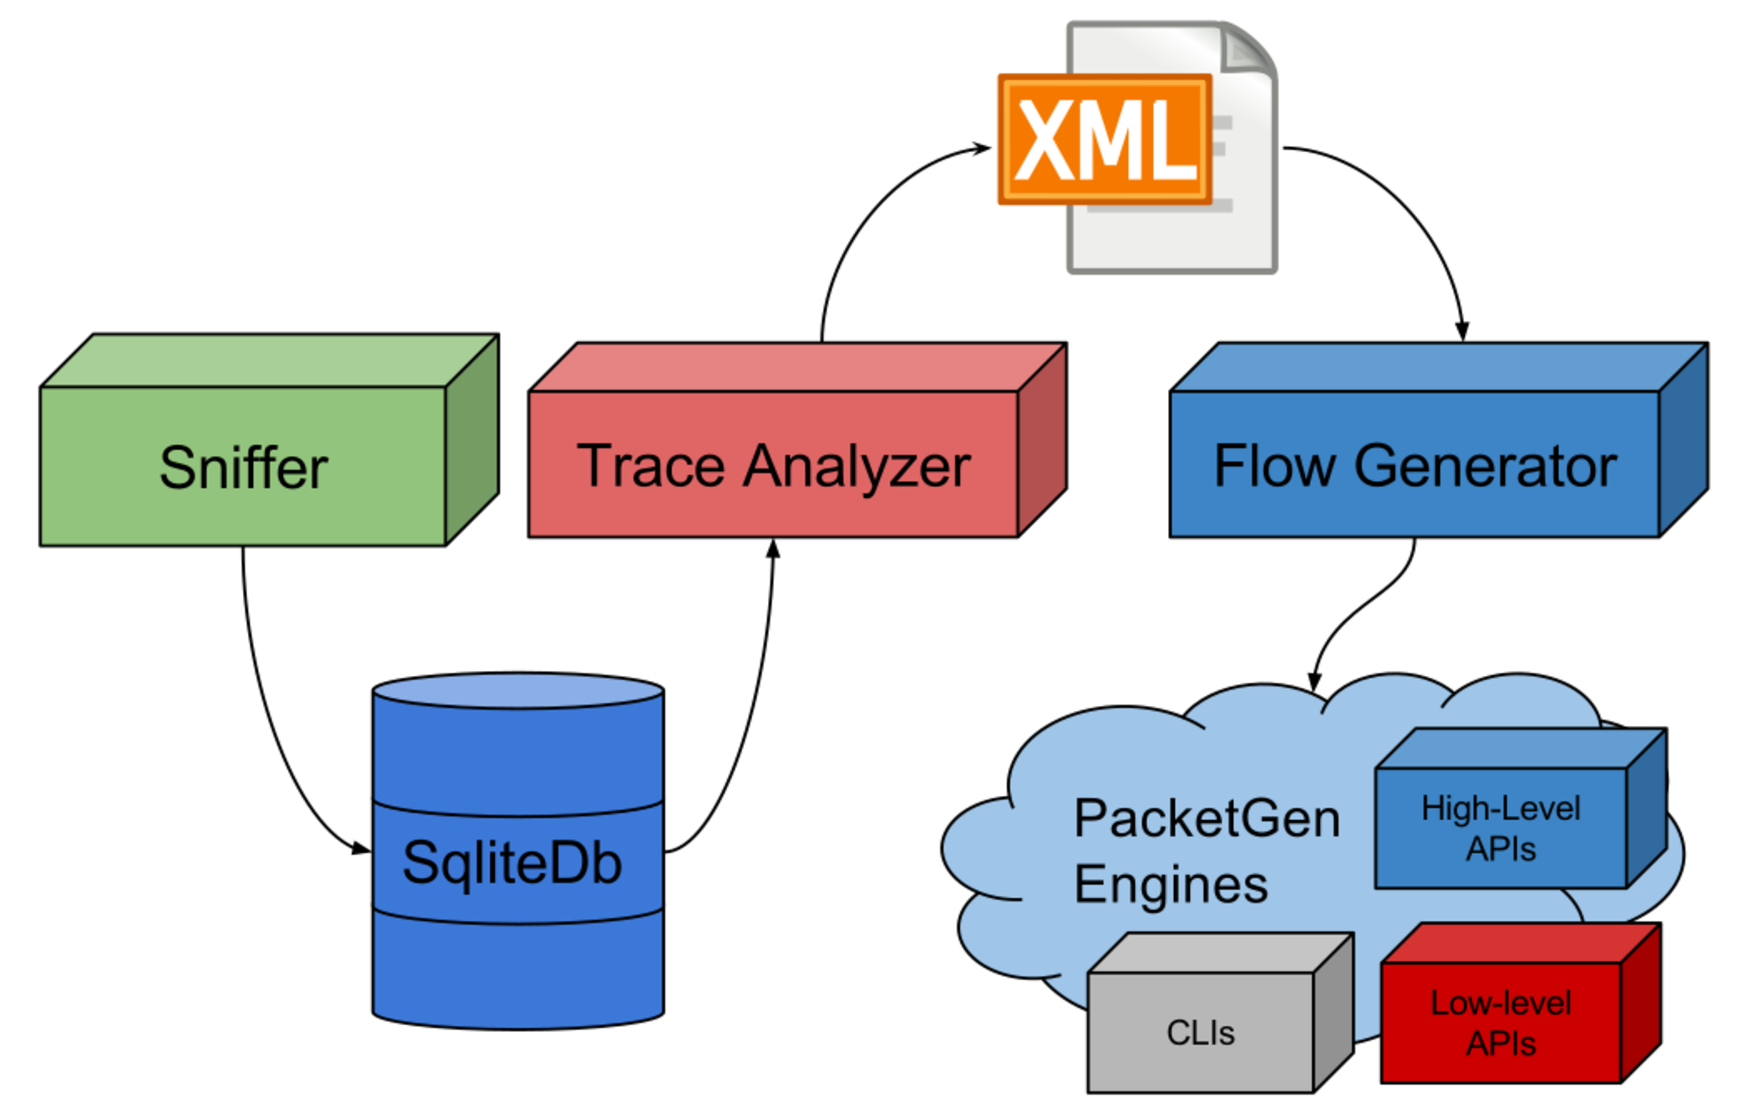
\includegraphics[height=2.7in]{figures/ch3/architecture-diagram}
        \caption{Architecture of SIMITAR}
    \label{fig:architecture}
\end{figure*}

%%%%%%%%%%%%%%%%%%%%%%%%%%%%%%%%%%%%%%%%%%%%%%%%%%%%%%%%%%%%%%%%%%%%%%%%%%%%%%%%
\section{ \textit{Sniffer} }


A sniffer is a tool that can intercept and analyze internet packets from a given network interface. Our \textit{Sniffer} component collects network traffic data and classifies it into flows, storing it on an SQLite database. It uses header field matches to classify the flows, such as in SDN switches\cite{sdn-survey}. The fields used  are:

\begin{itemize}
\item Link Protocol
\item Network Protocol
\item Network Source and Destination Address
\item Transport Protocol
\item Transport Source and Destination Port
\end{itemize}


\begin{figure*}[ht!]
        \centering
        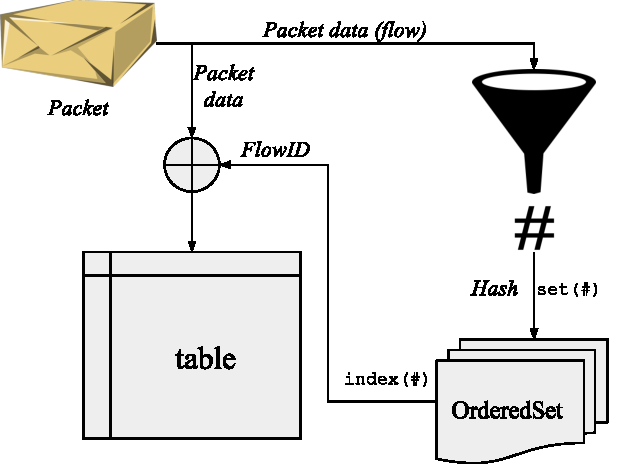
\includegraphics[height=2.5in]{figures/ch3/sniffer-classifier}
        \caption{SIMITAR's sniffer hash-based flow classification}
    \label{fig:sniffer}
\end{figure*}



We implemented the first version of this component in Shell Script (Bash). Tshark\cite{web-tshark} was used to extract header fields, and Awk to match the flows, and Sed/Awk to create the SQLite queries. This version was too slow to operate in real time on ethernet interfaces. On the other hand, this approach was fast to implement and enabled the implementation of the other components. The second and current version is in Python. This version used Pyshark\cite{web-pyshark} as a sniffer library.

The \textit{Sniffer} has a data structure we developed called \textit{OrderedSet}. A set is a list of elements with no repetition but does not keep track of the insertion order. Our \textit{OrderedSet} does. Also, it uses a 64 bit hash function from the \acrshort{FNV}\footnote{The collision probability of a good 64 bits hash function in a table with 10000 items is about of $2.71e-12$.} family. The listed header fields are inputs for a hash function. The hash value is added to the ordered set which returns its order (index on the \textit{OrderedSet}). We chose its value as packet \acrshort{flowID}.

%c++ http://ideone.com/F0V42m
As future improvements for this component, we propose a more efficient implementation in C++ and data visualization for the collected data. In this way, we can optimize packet processing. We discuss this in more depth in chapter~\ref{ch:conclusion}.

%%%%%%%%%%%%%%%%%%%%%%%%%%%%%%%%%%%%%%%%%%%%%%%%%%%%%%%%%%%%%%%%%%%%%%%%%%%%%%%%
\section{ \textit{SQLite database} }

\begin{figure*}[ht!]
        \centering
        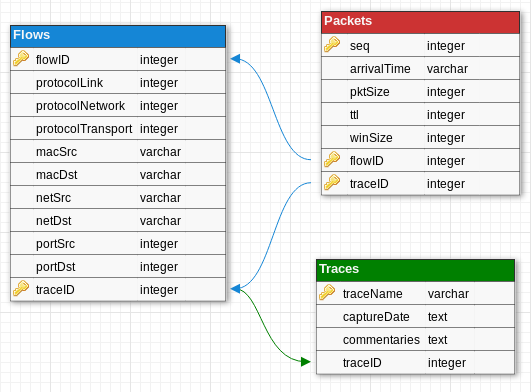
\includegraphics[height=3.0in]{figures/ch3/database-relational-model}
        \caption{SIMITAR's SQLite database relational model}
    \label{fig:simitar-database}
\end{figure*}




The database stores the collected raw data from the traces for further analysis. The \textit{Sniffer} records data on it and the  \textit{Trace Analyzer} reads. We choose an SQLite database because according to its specifications\cite{web-sqlite}, it fits our purposes well. It is simple and suitable for an amount of data smaller than terabytes. In figure~\ref{fig:simitar-database}, we present the relational model of our database, which stores a set of features extracted from packets, along with the flowID calculated by the \textit{Sniffer} component.


%%%%%%%%%%%%%%%%%%%%%%%%%%%%%%%%%%%%%%%%%%%%%%%%%%%%%%%%%%%%%%%%%%%%%%%%%%%%%%%%
\section{ \textit{Trace Analyzer} }


This module is the core of our project. It creates a trace model via the analysis of the collected data. The \textit{Trace Analyzer} has the task to learn these features from raw trace data (stored in the SQLite database) and generate an XML file to store a parameterized model. A \textit{Compact Trace Descriptor} (CTD) acts as a human and machine-readable file, which describes a traffic trace through a set of flows, each of them represented by a set of parameters, such as header information and analytical models. In figure~\ref{fig:CTD-diagram} we show a directory diagram of a CDT file. It has many flow fields, and each one contains each estimated parameter . We will now describe how we constructed it.


\begin{figure}
\centering
\subfloat[]{
  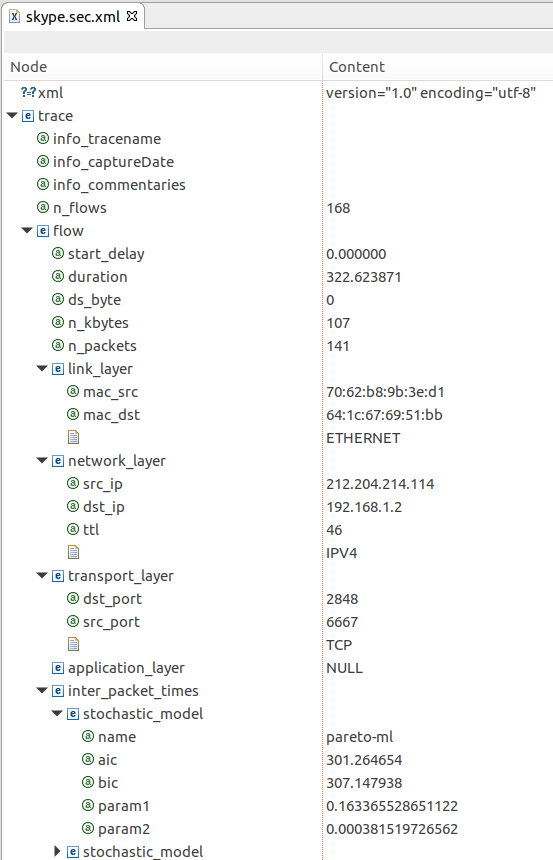
\includegraphics[height=4.in]{figures/ch3/cdt1}
}
\subfloat[]{
  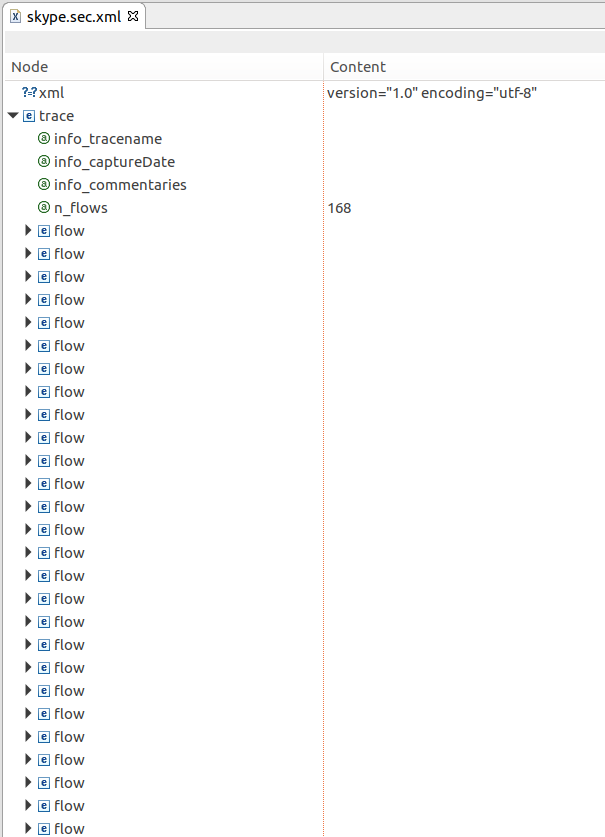
\includegraphics[height=4.in]{figures/ch3/cdt2}
}
\caption{Directory diagram of the schema of a Compact Trace Descriptor (CDT) file. On the left, we present a dissected flow, and on the right a set of flows.}
\label{fig:CTD-diagram}
\end{figure}


%%%%%%%%%%%%%%%%%%%%%%%%%%%%%%%%%%%%%%%%%%%%%%%%%%%%%%%%%%%%%%%%%%%%%%%%%%%%%%%%
\subsection{Flow features}

We measured some flow-features directly from data. They are:

\begin{itemize}
\item Flow-level properties like duration of flow, start delay, number of packets per flow, number of KBytes per flow;
\item Header fields, like protocols, QoS fields, ports, and addresses.
\end{itemize}

Each one of these parameters is unique to each flow. Other features like packet-size distribution and inter-packet times follow probability distributions. To represent these characteristics, we used sets of stochastic-based models.

%%%%%%%%%%%%%%%%%%%%%%%%%%%%%%%%%%%%%%%%%%%%%%%%%%%%%%%%%%%%%%%%%%%%%%%%%%%%%%%%
\subsection{Inter-Packet Times}


\begin{figure*}[ht!]
    \centering
    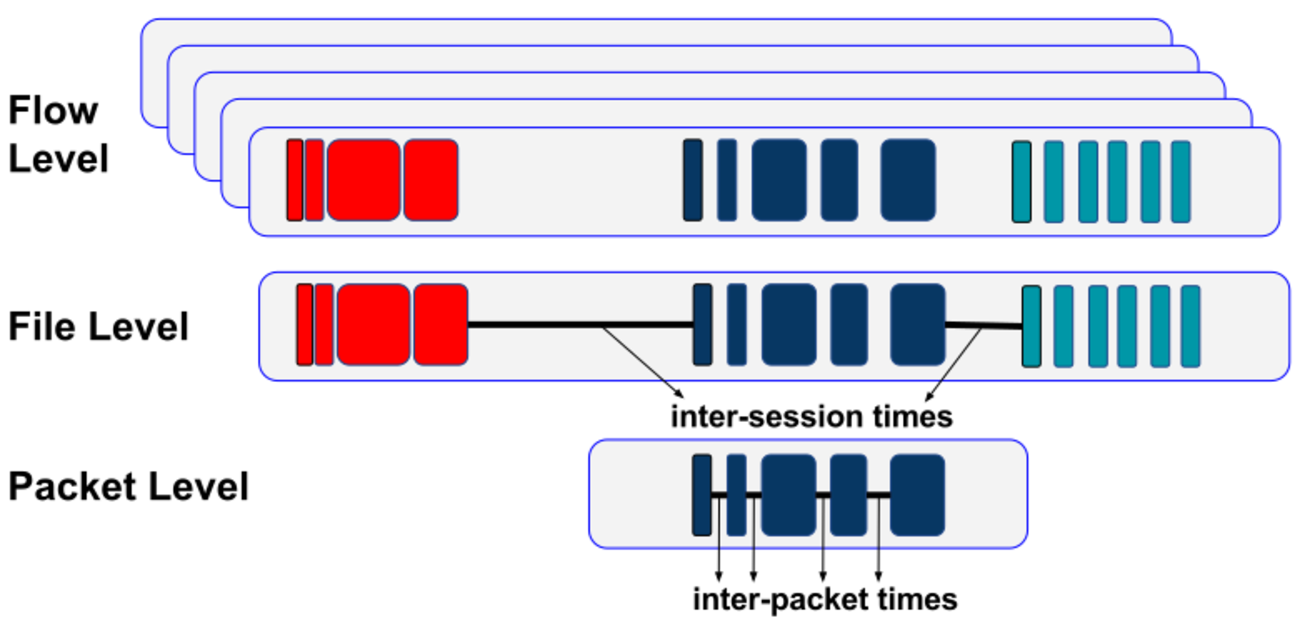
\includegraphics[height=2.0in]{figures/ch3/modified-harpoon-model}
    \caption{The schema of the modified version of the Harpoon algorithm we adopt on SIMITAR.}
    \label{fig:modified-harpoon-model}
\end{figure*}


To represent inter-packet times, we adopted a modified version of the Harpoon’s traffic model. An in-depth explanation of the original model can be found at  \cite{harpoon-paper} and \cite{harpoon-validation}. Harpoon uses a definition of each level, based on the measurement of \acrshort{SYN} and \acrshort{ACK} TCP flags. It uses TCP flags (SYN) to classify packets at different levels, naming their file, session, and user level. We chose to estimate these values, based on inter-packet times only. The distinction is made based on the time delay between packets. For our purposes, the advantage of our strategy is that the evaluation of the packet-train is not attached to a specific header field so that we can define packet trains for any flow. We illustrate this behavior in figure~\ref{fig:modified-harpoon-model}.

In our algorithm, we defined three different layers of data transference to model and control: \textit{file}, \textit{session}, and \textit{flow}. For SIMITAR, a file is a sequence of consecutive packets transmitted continuously, without a long interruption of traffic. A file can be, for example, packets from a download, a UDP connection or a single \acrshort{ICMP} echo packet. The session-layer refers to a sequence of multiple files transmitted between a source and a destination, belonging to the same flow. The flow level refers to the conjunction of flows, as classified by the \textit{Sniffer}. Now, we will explain SIMITAR operation for each layer.

In the \textbf{flow-layer}, the \textit{Trace Analyzer}  loads the flow arrival times from the database and calculates the inter-packet times within the flow context. At the session layer, we used a deterministic approach for evaluating file transference time and times between files: ON/OFF times sequence for packet trains. We chose a deterministic model because in this way we can express diurnal behavior. We developed an algorithm called \texttt{calcOnOff} that estimates these times. It also determines the number of packets and bytes transferred for each file. Since the ON times will serve as input for actual traffic generators, we defined a minimum acceptable time for on periods equal to 100 ms. ON times can be arbitrary and small, and they could be incompatible with acceptable ON periods for traffic generators. Also in the case of just one packet, the ON time would be zero. So  a minimum acceptable time was set to solve these issues. The OFF times, on the other hand, are defined by the constant \texttt{session\_cut\_time}\footnote{In the code it is called \texttt{DataProcessor::m\_session\_cut\_time} }. If the time between two packets of the same flow is greater than \texttt{session\_cut\_time}, we consider them belonging to a different file, so this time is a session OFF time. In this case, we use the same value of the constant \textit{Request and Response timeout} of Swing\cite{swing-paper} for the \texttt{session\_cut\_time}: 30 seconds. The control of ON/OFF periods in the traffic generation is made by the \textit{Flow Generator} component\footnote{This control is made by the class \texttt{NetworkFlow}}.

In the \textbf{file-layer}, we modeled the inter-packet times at the file level. We selected all times smaller than \texttt{session\_cut\_time} 9, and all files within the same flow were considered to follow the same model. We delegated the control of the inter-packet times to the underlying packet generator engine. We ordered them, from the best to the worst. Currently, we are using eight different stochastic functions parameterizations. We display each of them in table~\ref{tab:parameterizations-sumary} .

\begin{table}[ht!]
	\centering
	\caption{Functions and parameterizations used by SIMITAR}
		\begin{tabular}{c c c c}
			\toprule
			\textbf{Function} & Linear Regression & Maximum Likelihood & Empirical\footnotemark \\
			\midrule
			Weibull         & $\checkmark$    &                  &                  \\
			Normal             &                  &                  &  $\checkmark$    \\
			Exponential      & $\checkmark$    &                  &  $\checkmark$    \\
			Pareto          & $\checkmark$    & $\checkmark$    &                  \\
			Cauchy          & $\checkmark$    &                  &                  \\
			Constant          &                 &                  & $\checkmark$    \\
			\bottomrule
		\end{tabular}
		\label{tab:parameterizations-sumary}
\end{table}
\footnotetext{Empirical estimation, by calculation of the avarge, and standard deviation} 


From the functions presented in the first column in table~\ref{tab:parameterizations-sumary}, Weibull, Pareto, and Cauchy are heavy-tailed (and self-similar processes). However, if the flow has less than 30 packets, just the constant model is evaluated. It is because numerical methods gave poor results if the data sample is small. We sorted these models according to the Akaike Information Criterion (AIC) as default\cite{sourcesonoff-paper}\cite{bic-aic-comparision}. This methodology is explained in-depth in chapter~\ref{ch:modeling-evaluation} and illustrated in figure 10.  All these constants and modes of operation are modifiable via command-line options.

\begin{figure*}[ht!]
    \centering
    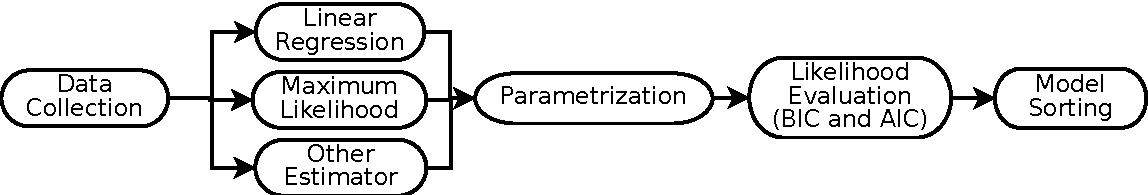
\includegraphics[height=0.9in]{figures/ch3/simitar-parametrization}
    \caption{Diagram of parameterization and model selection for inter-packet times and inter-file times.}
    \label{fig:model-parameterization}
\end{figure*}

%%%%%%%%%%%%%%%%%%%%%%%%%%%%%%%%%%%%%%%%%%%%%%%%%%%%%%%%%%%%%%%%%%%%%%%%%%%%%%%%
\subsection{Packet Sizes}


Our approach for the packet size was much simpler. Since the majority of packet size distributions found in real measurements are bi-modal\cite{packet-distribution-model}\cite{sourcesonoff-paper}\cite{udp-flows-model}, we first sorted all packet sizes of flow into two modes. We defined a packet-size cut value of 750 bytes, the same value adopted by\cite{udp-flows-model}.

We knew how many packets each mode has, and then we fitted a model to it. We use three stochastic models: constant, exponential and normal. Since self-similarity does not make sense for packet-sizes, we prefered to use just the simpler models. When there was no packet for a model, we set a flag \texttt{NO\_MODEL}, and when there was only a single packet, we used the constant model. Then we calculated the $BIC$ and $AIC$ for each, but we decided to set the constant model as the first.

As is possible to see in many works\cite{packet-distribution-model} \cite{udp-flows-model}, since the standard deviation of each mode tends to be small, constant fittings give good approximations. Also, it is computationally cheaper for the traffic generated than the other models, since no calculation is needed for each packet sent. Since both $AIC$ and $BIC$ criteria will always select the constant model as the worst, we decided to ignore this.

%%%%%%%%%%%%%%%%%%%%%%%%%%%%%%%%%%%%%%%%%%%%%%%%%%%%%%%%%%%%%%%%%%%%%%%%%%%%%%%%
\subsection{ \textit{Compact Trace Descriptor} }


An example of the final result of all the methods is presented in the XML code below. The code illustrates a single flow from a \textit{Compact Trace Descriptor}(CDT) file. The inter-packet times' models are on tags "\texttt{inter\_packet\_times}" and the packet trains models on tags "\texttt{session\_times}". All the times are in seconds, and "\texttt{inf}" represents infinity. The protocol of each layer is on the data field for each tag. 


\begin{minted}[frame=single,
               framesep=3mm,
               linenos=true,
               xleftmargin=21pt,
               tabsize=4,
               fontsize=\scriptsize, 
               breaklines=true]{xml}
    <flow start_delay="0.144400" duration="317.744333" ds_byte="0" n_kbytes="40" n_packets="344">
        <link_layer mac_src="64:1c:67:69:51:bb" mac_dst="70:62:b8:9b:3e:d1">ETHERNET</link_layer>
        <network_layer src_ip="192.168.1.1" dst_ip="192.168.1.2" ttl="64">IPV4</network_layer>
        <transport_layer dst_port="2128" src_port="53">UDP</transport_layer>
        <application_layer>DNS</application_layer>
        <inter_packet_times>
            <stochastic_model name="pareto-ml" aic="-1165.310696" bic="-1157.646931" param1="0.405085202535192" param2="0.002272655895996"/>
            <stochastic_model name="pareto-lr" aic="-454.049749" bic="-446.385984" param1="0.061065000000000" param2="0.002272655895996"/>
            <stochastic_model name="weibull" aic="-246.882037" bic="-239.218273" param1="0.120355000000000" param2="0.001629000000000"/>
            <stochastic_model name="exponential-me" aic="486.370061" bic="494.033826" param1="1.340057495455104" param2="0.000000000000000"/>
            <stochastic_model name="normal" aic="1629.370900" bic="1637.034665" param1="0.746236637899171" param2="2.626808289821357"/>
            <stochastic_model name="exponential-lr" aic="3166.816047" bic="3174.479812" param1="0.009752000000000" param2="0.000000000000000"/>
            <stochastic_model name="cauchy" aic="31737.418442" bic="31745.082207" param1="0.000000000000194" param2="-3152.827055696396656"/>
            <stochastic_model name="constant" aic="inf" bic="inf" param1="0.746236637899171" param2="0.000000000000000"/>
        </inter_packet_times>
        <session_times on_times="29.22199798,73.40390396,151.84077454" off_times="30.85738373,32.42027283" n_packets="19,103,222" n_bytes="2272,12399,26689"/>
        <packet_sizes n_packets="344" n_kbytes="40">
            <ps_mode1 n_packets="344" n_kbytes="40">
                <stochastic_model name="constant" aic="inf" bic="inf" param1="120.232558" param2="0.000000"/>
                <stochastic_model name="normal" aic="2926.106952" bic="2933.788235" param1="120.232558" param2="16.941453"/>
                <stochastic_model name="exponential-me" aic="3987.126362" bic="3994.807645" param1="0.008317" param2="0.000000"/>
            </ps_mode1>
            <ps_mode2 n_packets="0" n_kbytes="0">
                <stochastic_model name="no-model-selected" aic="inf" bic="inf" param1="0.000000" param2="0.000000"/>
            </ps_mode2>
        </packet_sizes>
    </flow>
\end{minted}


%%%%%%%%%%%%%%%%%%%%%%%%%%%%%%%%%%%%%%%%%%%%%%%%%%%%%%%%%%%%%%%%%%%%%%%%%%%%%%%%
\section{ \textit{Flow Generator} }

\begin{figure*}[pht!]
    \centering
    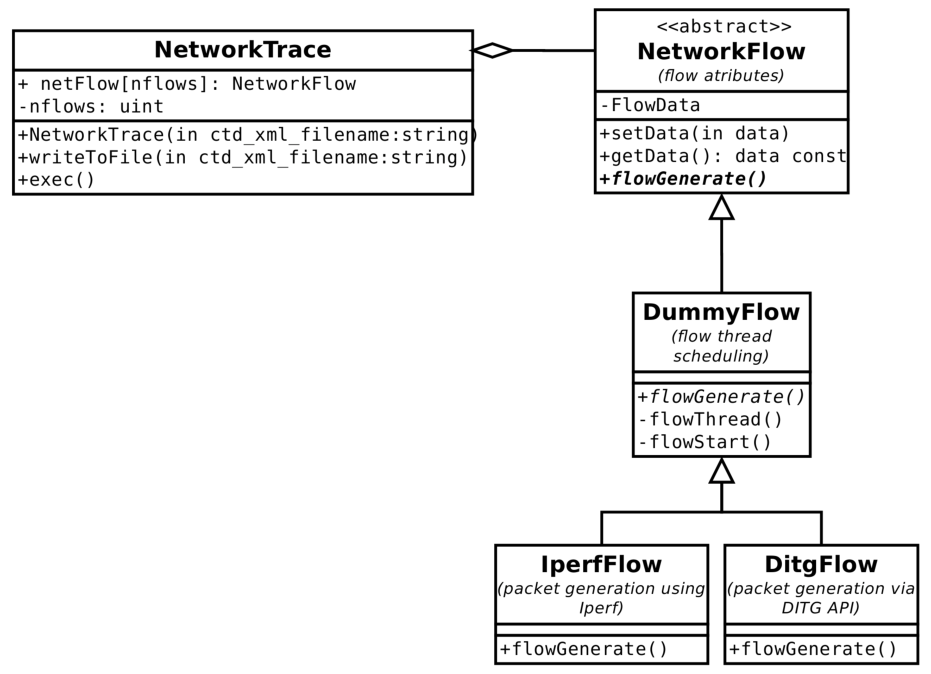
\includegraphics[height=3.0in]{figures/ch3/trace-flow}
    \caption{Class hierarchy of NetworkTrace and NetworkFlow, which enables the abstraction of the traffic generation model of the packet generation engine.}
    \label{fig:network-trace-flow-class-diagram}
\end{figure*}

\begin{figure*}[pht!]
    \centering
    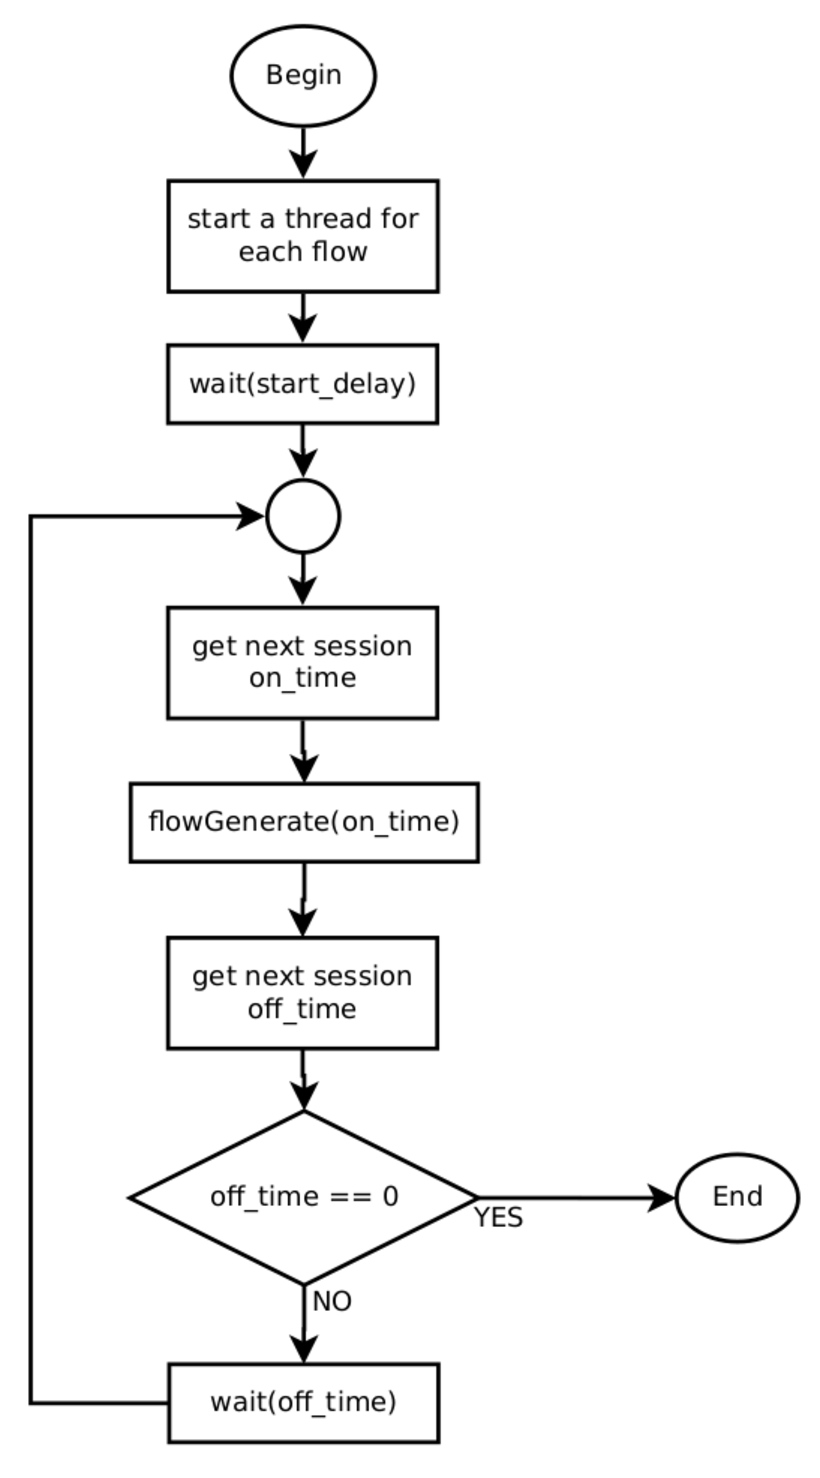
\includegraphics[height=4.5in]{figures/ch3/alg-simplified-harpoon}
    \caption{Simplified-harpoon emission algorithm}
    \label{fig:alg-simplified-harpoon}
\end{figure*}


\begin{figure*}[pht!]
    \centering
    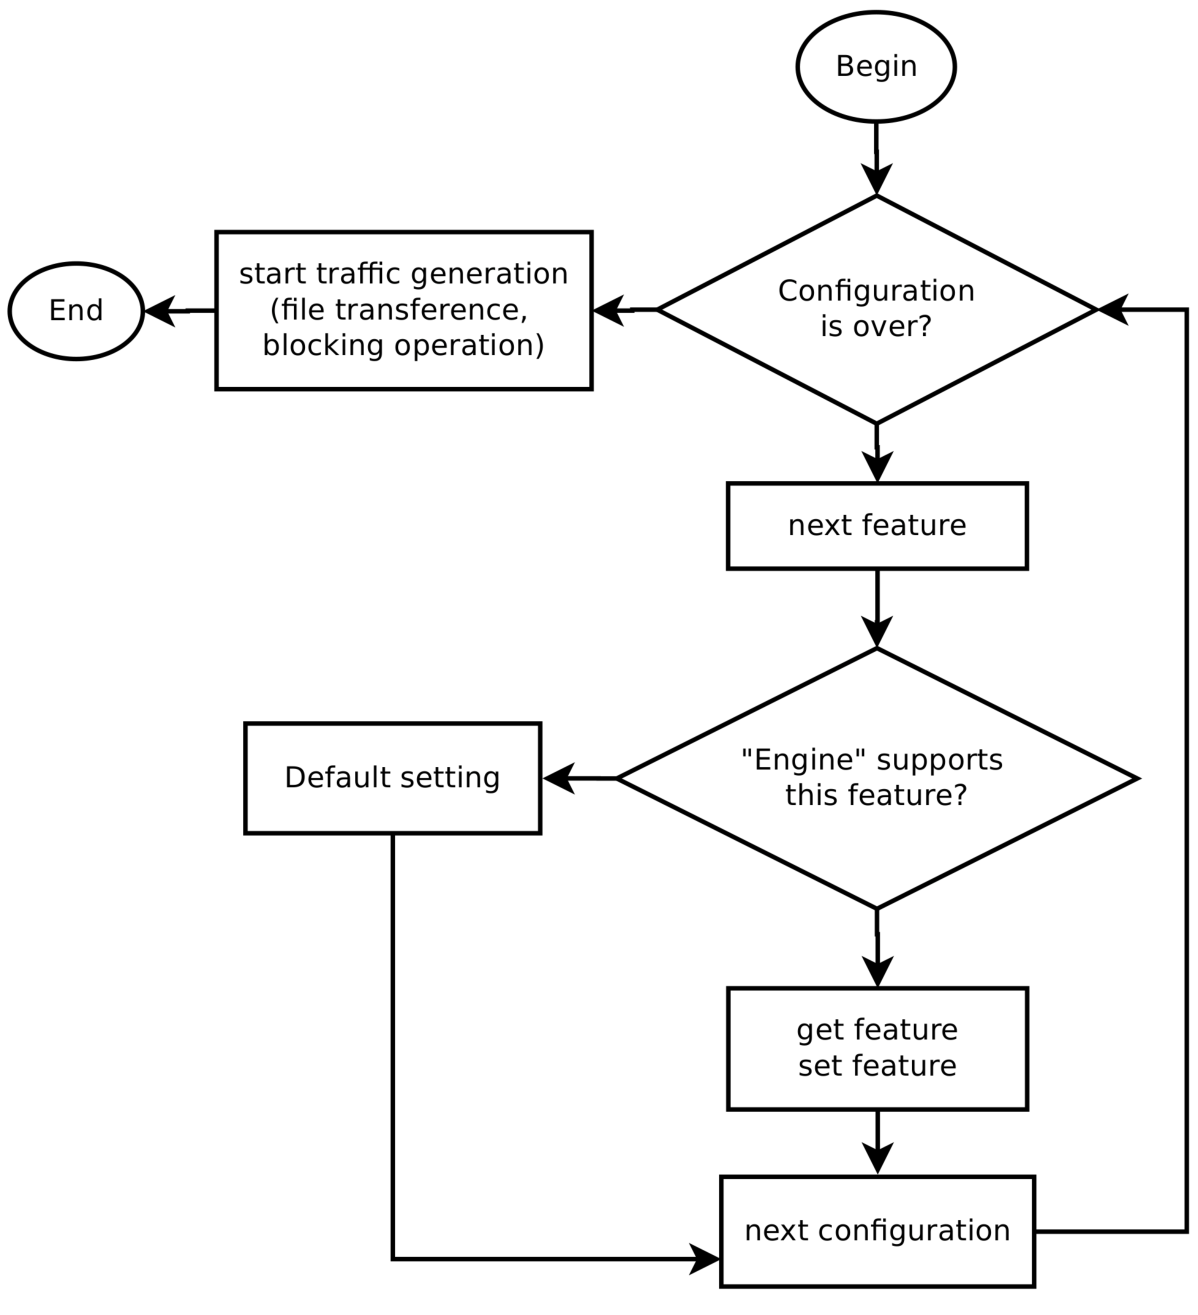
\includegraphics[height=4.0in]{figures/ch3/alg-traffic-engine-config}
    \caption{Packet engine configuration method}
    \label{fig:alg-traffic-engine-config}
\end{figure*}



The \textit{Flow Generator} handles the data on the \textit{Compact Trace Descriptor} file, and is used to retrieve parameters for traffic generation. It crafts and controls each flow in a separate thread. We have already implemented this component using Iperf and Libtins(C++ API)\cite{web-libtins} as packet generators. It must follow the class hierarchy as presented in figure~\ref{fig:network-trace-flow-class-diagram}. This component was designed using the factory design pattern, to simplify its expansion and support\footnote{
If the user wants to introduce support for a new packet generator engine, he has to implement a derived class of \texttt{DummyFlow}, such as in figure~\ref{fig:network-trace-flow-class-diagram}. In the current release of SIMITAR, we already have \texttt{IperfFlow} and \texttt{TinsFlow}, and \texttt{DitgFlow}. This new class needs to be static, and the support must be implemented on the factory \texttt{NetworkFlowFactory}.
For closed loop packet-crafters (the ones that need to establish a connection to generate traffic), two methods must be implemented: \texttt{flowGenerate()} and \texttt{server()}. \texttt{flowGenerate()} is responsible for sending a single file, as defined on de figure~\ref{fig:modified-harpoon-model}. The \texttt{server()} methods must implement the reception of $n$ files. For open-loop packet crafters (the ones whose just inject packets but do not establishes a connection), such as the one we implemented using Libtins, does not need the server-side implemented. }


This component itself is a multi-layer workload generator according to the typing introduced in chapter~\ref{ch:literature-review}\footnote{Since it works both at packet and flow level, but does not work at application level yet.}. At the flow-level, SIMITAR controls each flow using the algorithm in figure~\ref{fig:alg-simplified-harpoon}. This algorithm handles our model as defined in figure~\ref{fig:modified-harpoon-model}. This procedure is independent of the underlying packet crafting tool used. It starts a \textit{thread} for each flow in the \textit{Compact Trace Descriptor}, and then the thread sleeps for \texttt{start\_delay} seconds. The \texttt{start\_delay} is the arrival time of the first flow packet. Passed this time, it then calls the underlying packet generator tool (defined as command line argument), and passes to it the flowID, file ON time, number of packets and number of bytes to be sent (file size), and network interface. Then it sleeps until the next session OFF time. When the list of ON/OFF times from the flow is over, the thread ends.


At the packet level, SIMITAR configures the packet-generator tool to send a \textit{file}, as defined in figure~\ref{fig:modified-harpoon-model}. This method must use the available parameters, attributes and \textit{getters} to configure and generate thread-safe traffic using the method \texttt{flowGenerate()}. The \textit{file} configuration must follow figure~\ref{fig:alg-traffic-engine-config}. Down below we present a simple code of how the D-ITG API can be used to generate packet-level traffic. A more complex configuration is possible, but it serves to illustrate the procedure. We call this concept \textit{Flow Generation Programming}. Its API documentation is available at the D-ITG website\footnote{\href{http://www.grid.unina.it/software/ITG/manual/index.html\#SECTION00047000000000000000}{http://www.grid.unina.it/software/ITG/manual/index.html\#SECTION00047000000000000000}}.

\begin{minted}[frame=single,
               framesep=3mm,
               linenos=true,
               xleftmargin=21pt,
               tabsize=4,
               fontsize=\scriptsize, 
               breaklines=true]{c++}


// This implementation is just a simplified version to illustrate the procedure.
void DitgFlow::flowGenerate(const counter& flowId, const time_sec& onTime, const uint& npackets, const uint& nbytes,  const string& netInterface)
{
    // create command to generate the traffic
    std::string strCommand;
    std::string localhost = getNetworkSrcAddr(); 
    strCommand += " -t " + std::to_string(onTime); 
    strCommand += " -k " + std::to_string(nbytes / 1024);
    strCommand += " -a " + getNetworkDstAddr();
    
    // configure protocol
    if (this->getTransportProtocol() == PROTOCOL__TCP)
        strCommand += " -T TCP -D ";
    else if (this->getTransportProtocol() == PROTOCOL__UDP)
        strCommand += " -T UDP ";
    else if (this->getTransportProtocol() == PROTOCOL__ICMP)
        strCommand += " -T ICMP ";
        
    //configure inter-packet time model, just Weibull or Constant
    StochasticModelFit idtModel;
    for(uint i = 0;;i++)
    {    
        idtModel = this->getInterDepertureTimeModel(i);
        if(idtModel.modelName() == WEIBULL)
        {
            strCommand += " -W " + std::to_string(idtModel.param1()) + " " + std::to_string(idtModel.param2());
            break;
        }
        else if ( idtModel.modelName() == CONSTANT)
        {
            strCommand += " -C " + std::to_string(nbytes/(1024*onTime));
            break;
        }
    }
    
    // it uses C strings as arguments
    // it is not blocking, so it must block until finishes
    int rc = DITGsend(localhost.c_str(), command.c_str()); // D-ITG API
    usleep(onTime*10e6); // D-ITG uses miliseconds as time unity
    if (rc != 0)
    {
        PLOG_ERROR << "DITGsend() return value was" << rc ; // our log macro for erros
        exit(EXIT_FAILURE);
    }
}
\end{minted}


%%%%%%%%%%%%%%%%%%%%%%%%%%%%%%%%%%%%%%%%%%%%%%%%%%%%%%%%%%%%%%%%%%%%%%%%%%%%%%%%
\section{Network Packet Generator}


A network packet generator is a tool or library that should provide its API or script interface for the \textit{Flow Generator} component. With this engine, the user must be able to send packets and control attributes such as sending time, bandwidth, number of packets, protocols, and so on. This means, any available parameter form the \textit{Compact Trace Descriptor}.


%%%%%%%%%%%%%%%%%%%%%%%%%%%%%%%%%%%%%%%%%%%%%%%%%%%%%%%%%%%%%%%%%%%%%%%%%%%%%%%%
\section{Usage and Use Cases}


SIMITAR is composed of three main command-line applications, whose give command line access to the \textit{Sniffer}, \textit{Trace Analyzer} and \textit{Flow Generator}, respectively:
\begin{itemize}
\item \texttt{sniffer-cli.py};
\item \texttt{trace-analyzer};
\item \texttt{simitar-gen} (the actual traffic generator). 
\end{itemize}

Below we show some usage commands of SIMITAR’s components. The \texttt{sniffer-cli.py} application creates a new trace entry on the database using the command option new. Then the \textit{Trace Analyzer} can create a \textit{Compact Trace Descriptor} using the same trace entry. We can change the constants used by the \textit{Trace Analyzer} by the command line option. As a traffic generator (\texttt{simitar-gen}), SIMITAR may work as a client or a server. Working as a server is necessary for closed-loop packet-generator engines; tools that require establishing a connection before generating the traffic, such as Iperf and D-ITG. It will just work passively. Working as a client it is acting as a traffic emitter. Open loop packet-crafter tools such as Libtins do not require server operation to send the traffic. In the case of closed-loop tools, the destination IP addresses must be explicitly given in the command line by the options \texttt{--dst-list-ip} or \texttt{--dst-ip}.


\begin{minted}[frame=single,
               framesep=3mm,
               linenos=true,
               xleftmargin=21pt,
               tabsize=4,
               fontsize=\scriptsize, 
               breaklines=true]{bash}

# @ SIMITAR/, load enviroment variables
source data/config/simitar-workspace-config.sh

# @ SIMITAR/sniffer/, execute to sniff the eth0 interface, and create a trace entry called "intrig" in the database
./sniffer-cli.py new intrig live eth0

# @ SIMITAR/sniffer/, execute this command to list all traces recorded in the database
./sniffer-cli.py list

# @ SIMITAR/trace-analyzer/, execute this command to create two Compact Trace Descriptors, called intrig.ms.xml and intrig.sec.xml. The first is parameterized using milliseconds, and de second uses seconds as time unity.
./trace-analyzer --trace intrig

# @ SIMITAR/simitar-gen/, execute these commands to generate traffic using the intrig.sec.xml compact trace descriptor. It is stored at the directory "../data/xml/". 
# Libtins
./simitar-gen --tool tins --mode client --ether eth0 --xml ../data/xml/intrig.sec.xml 
# Iperf
./simitar-gen --tool iperf --mode client --ether eth0 --xml ../data/xml/intrig.sec.xml --dst-ip 10.0.0.2
./simitar-gen --tool iperf --mode server --ether eth0 --xml ../data/xml/intrig.sec.xml

\end{minted}


\begin{figure*}[ht!]
    \centering
    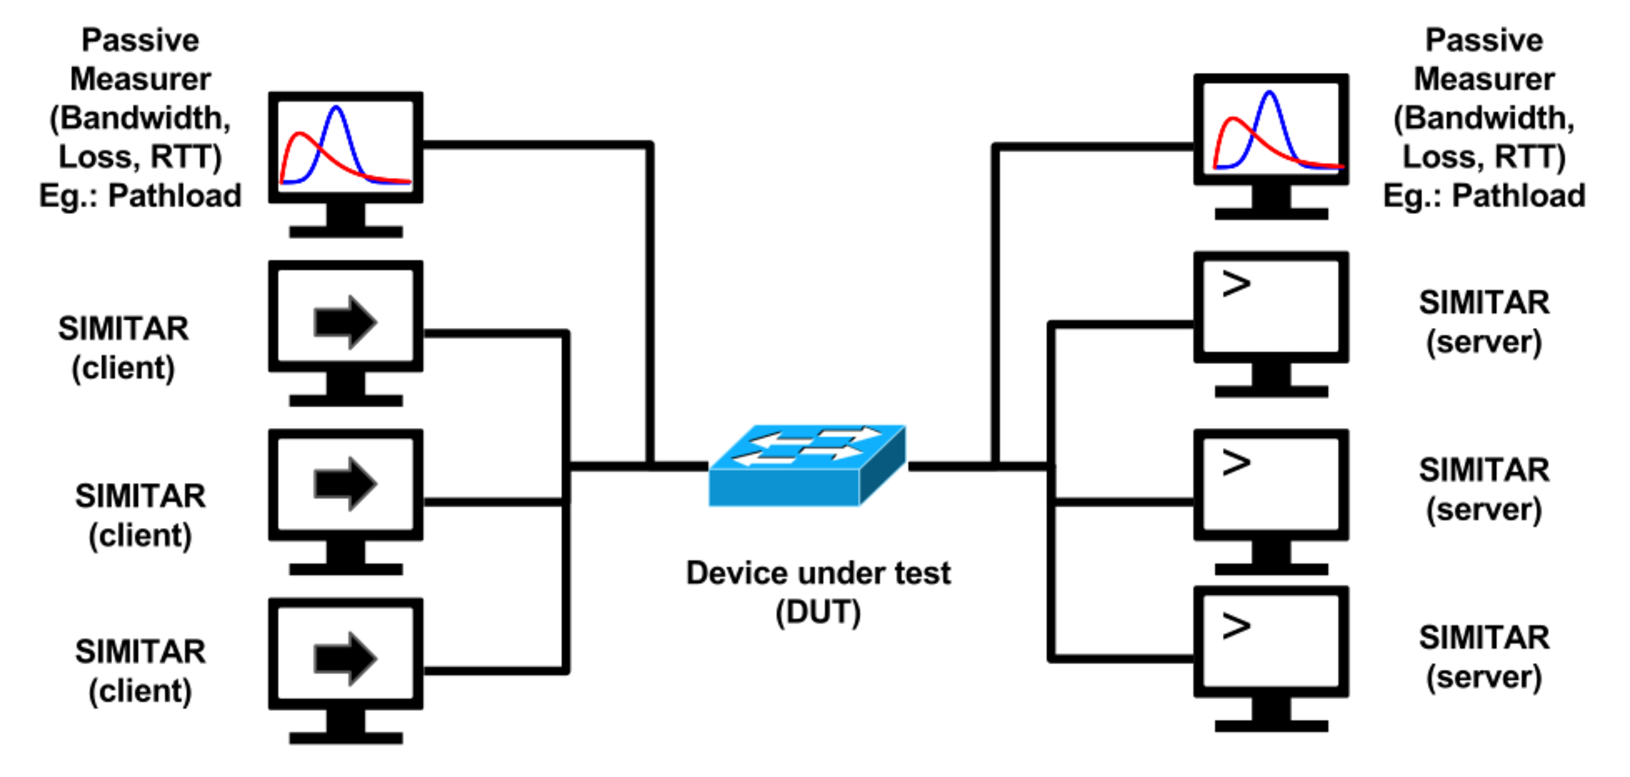
\includegraphics[height=2.4in]{figures/ch3/use-case}
    \caption{Use case example of SIMITAR}
    \label{fig:use-case}
\end{figure*}



Figure~\ref{fig:use-case} shows an example of a use case. A device under test can be stressed using a combination of traffic generated by many clients and server pairs. In the case of an open-loop packet generator tool (such as in the Libtins implementation), the servers and clients pairs are not necessary. Using passive network measures, such as Pathload\cite{web-pathload} and pathChirp\cite{swing-paper}\cite{web-pathchirp}, it is possible to measure statistics from the device under tests.
